\documentclass[a4paper]{article}
% Leave uncommented if the LaTeX file is uploaded to arXiv.org
\pdfoutput=1
\pdfminorversion=7

% Packages
\usepackage{arxiv}
\usepackage[colorlinks=true,linkcolor=cyan,citecolor=cyan]{hyperref}
\usepackage[numbers]{natbib}
\usepackage{authblk}
\usepackage{graphicx}
\usepackage{amsmath}
\usepackage{amssymb}
\usepackage{epstopdf}
\usepackage{comment}
\usepackage{xcolor}
\usepackage{float}
\usepackage{doi}

\title{\boldmath Magnetic properties of finite temperature primordial electron-positron plasma}

% Author Orcid ID: Define per author
\newcommand{\orcA}{0000-0001-8217-1484}
\newcommand{\orcB}{0000-0001-5038-8427}
\newcommand{\orcC}{0000-0001-5474-2649}

\author{Andrew Steinmetz\orc{\orcC}\thanks{Correspondence: \texttt{ajsteinmetz@arizona.edu}}, Cheng Tao Yang\orc{\orcB}, and Johann Rafelski\orc{\orcA}\\ Department of Physics, The University of Arizona, Tucson, AZ 85721, USA}

\begin{document}

\maketitle

\begin{abstract}
    We explore the possibility of magnetization within the primordial electron-positron plasma in the temperature range $2,000\keV>T>20\keV$ where the $e^{+}e^{-}$ pair density was up to $10^{9}$ greater than the baryon density. We suggest that primordial magnetization within the plasma is driven by spin paramagnetism. At these high densities, strong dampening by internal scattering needs to be included in any study of magneto-hydrodynamic flow. The rapid disappearance of $e^{+}e^{-}$ at temperature $T\simeq20\keV$ occurs much faster than the corresponding drop in temperature.
\end{abstract}

\keywords{early universe cosmology \and magnetization \and electron-positron plasma \and intergalactic magnetic fields}

%%%%%%%%%%%%%%%%%%%%%%%%%%%%%%%%%%%%%%%
\section{Introduction}\label{sec:introduction}
\noindent Macroscopic domains of magnetic fields have been found: around compact objects (stars, planets, etc...), between stars, within galaxies, between galaxies in clusters, and surprisingly in the deep extra-galactic void spaces where little matter exists. Therefore we search for a common mechanism that could produce the magnetic diversity we see in today's contemporary universe.

In the early universe above temperature $T>20\keV$ there was an gargantuan density of electron-positron pairs which rapidly vanished. We explore the possibility that this phenomenon was responsible for generating primordial magnetic fields in the universe. At higher electron-positron pair densities, spin paramagnetism is dominant over the Landau orbital diamagnetism of the gas. In this work, we seek to describe the magnetization of (and possible magnetogenesis within) the primordial electron-positron plasma as it underwent a rapid drop in density of $10^{9}$ relative to the baryon density in the temperature range $2,000\keV>T>20\keV$.

% Greatly compress discussion of other models and simply refer shortly to the multitude of other proposed mechanisms and models (provide already in existant references) and move on with out approach quickly.
Unlike electric fields which cannot be supported at large scales due to the charge neutrality of the universe, cosmic magnetic fields are easily generated~\cite{kronberg1994extragalactic,gaensler2004origin,durrer2013cosmological} by a variety of physicals phenomenon which are difficult to screen. These intergalactic magnetic fields (IGMF) present a challenge both experimentally and theoretically in that they are (a) difficult to measure and (b) difficult to explain using known physics. The bounds for IGMF at a coherent length scale of $1{\rm\ Mpc}$ are today~\cite{neronov2010evidence,taylor2011extragalactic,pshirkov2015new,vernstrom2021discovery}
\begin{align}
    \label{igmf}
    10^{-8}{\rm\ G}>\mathcal{B}_{\rm IGFM}>10^{-16}{\rm\ G}\,.
\end{align}
There are three conventional explanations~\cite{batista2021gammaray} for the existence of IGMF:
\begin{itemize}
    \item [1.] \textbf{Primordial fields} - Cosmic primordial magnetic fields (PMF) are produced in the universe before the recombination epoch possibly as far back as inflation. Such fields would arise from the cosmic-scale polarization of the early universe, phase transitions, or magnetogenesis from the breakdown of some unknown field.
    \item [2.] \textbf{Dynamo amplification} - Initially small \lq\lq seed\rq\rq\ magnetic fields dynamically reorganize charged matter fluids amplifying the total magnetic flux in a process called dynamo. Such seed fields may be primordial or astrophysical in origin.
    \item [3.] \textbf{Astrophysical sources} - Late times development of IGMF arises from stars, supernova and active galaxy nuclei (AGN) producing galactic outflows of charged matter which would contaminate and magnetize regions between galaxies.
\end{itemize}
Faraday rotation from distant radio AGN~\cite{pomakov2022redshift} suggest that neither dynamo nor astrophysical processes would sufficiently account for the presence of IGMF in the universe today if the IGMF strength was around the upper bound of ${\cal B}_{\rm IGMF}\simeq30-60{\rm\ nG}$ as found in~\cite{vernstrom2021discovery}. Such strong IGMFs would then require that at least some portion of the IGMF arise from primordial sources that predate the formation of stars and galaxies, or the CMB. It was shown by Jedamzik and Pogosian~\cite{jedamzik2020relieving} that the presence of ${\cal B}_{\rm PMF}\simeq0.1{\rm\ nG}$ could be sufficient to explain the Hubble tension. Such pre-recombination PMFs would lead to early universe baryon inhomogeneities which in turn would produce anisotropies in the CMB~\cite{jedamzik2013smallscale}. PMF strengths of around a tenth of a nanoGauss is also near the more stringent upper bound for PMFs found in~\cite{pshirkov2015new,jedamzik2019stringent}. Conversely, measurements of synchrotron radiation from \lq\lq blazar\rq\rq\ AGN whose jets are pointed towards the Earth provide the lower bound~\cite{neronov2010evidence,taylor2011extragalactic} on IGMFs seen in \req{igmf}.


Even if IGMFs are found to be produced by some mixture all three scenarios listed above, the existence of PMFs would be uniquely interesting because of their effects on (or generation within) the early universe primordial plasmas which populated the universe before recombination. We seek in this work to describe the influence PMFs had on the dense electron-positron $(e^{+}e^{-})$ plasma epoch in the temperature range $2\MeV>T>0.02\MeV$ in the early universe. We note that above temperature $T>85\keV$~\cite{rafelski2023short}, the $e^{+}e^{-}$ primordial plasma density exceeded that of the Sun's core density $n_{e}\simeq6\times10^{26}{\rm\ cm}^{-3}$~\cite{bahcall2001solar}. This combination of strong magnetic fields, high matter-antimatter density, and relatively high temperatures (far higher than the Sun's core temperature~\cite{castellani1997solar} of $T_{\odot}=1.37\keV$) make this era unique in cosmology and astrophysics. Other candidates include: inflationary magnetogenesis~\cite{subramanian2009magnetic}, electroweak transition~\cite{vachaspati2020progress}, QGP-hadronization eras~\cite{bali2011qcd}. It was found in~\cite{gopal2004generation} that the electron, proton, photon plasma of the immediate pre-recombination era generates (from density fluctuations) a tiny contemporary field of ${\cal B}\simeq10^{-30}{\rm\ G}$ far below the known IGMF bound or necessarily seed field size for dynamo. Due to cosmological redshift, and the conservation of magnetic flux over a comoving volume, PMFs would have extraordinary field strengths during the various primordial plasmas of the early universe subject to whatever temperature they were initially generated in.

%%%%%%%%%%%%%%%%%%%%%%%%%%%%%%%%%%%%%%%
\section{Electron-positron abundance}\label{sec:abundance}
%%%%%%%%%%%%%%%%%%%%%%%%%%%%%%%%%%%%%%%
\begin{figure}[h]
    \centering
    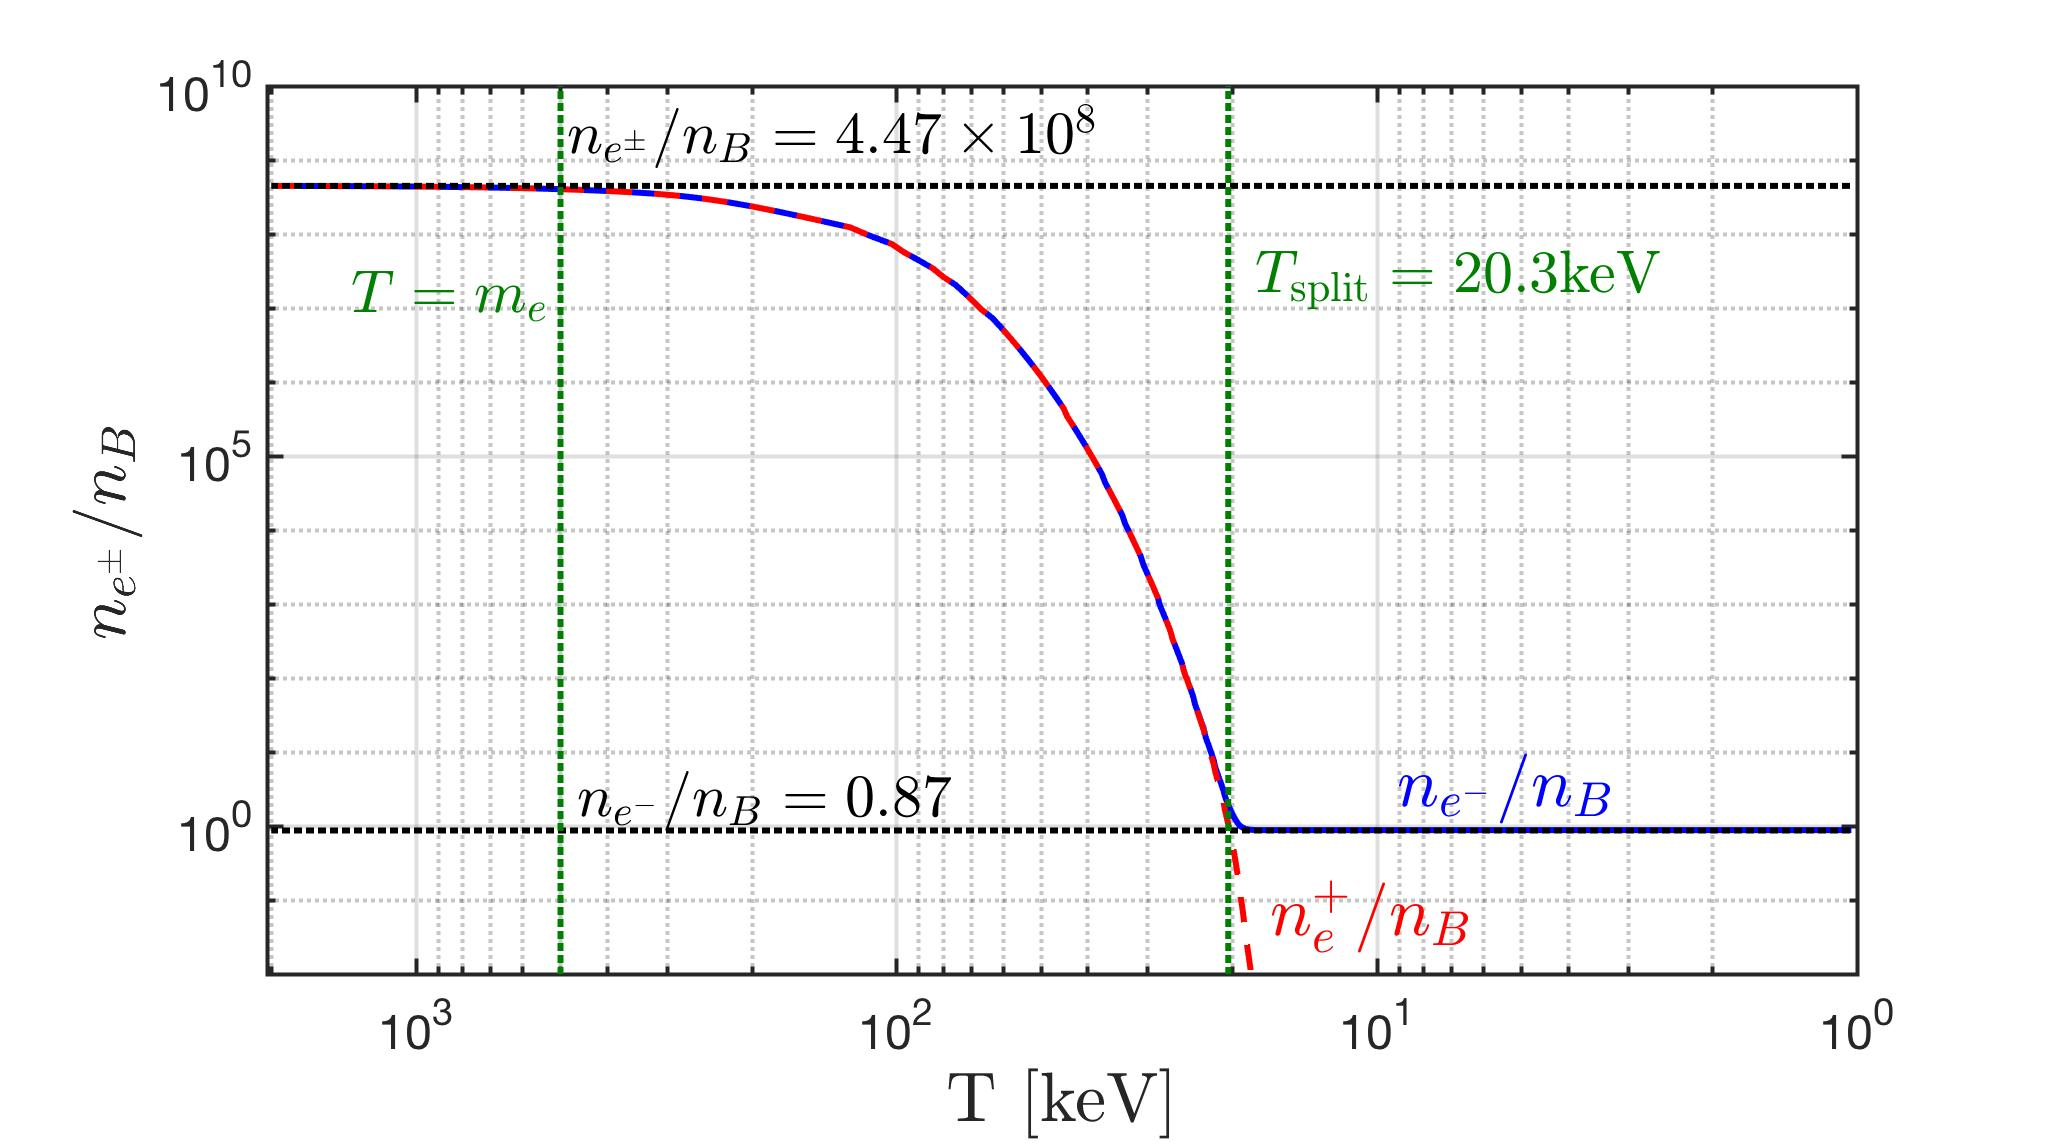
\includegraphics[width=\textwidth]{EEPlasmaDensityRatio.jpg}
    \caption{The light charged lepton-to-baryon ratio $n_{e^{\pm}}/n_{B}$ is plotted as a function of temperature. The electron-to-baryon ratio $n_{e^{-}}/n_{B}$ is shown as the solid blue line while the positron-to-baryon ratio $n_{e^{+}}/n_{B}$ is printed as the dashed red line. The two vertical dashed green lines denote temperatures $T=m_{e}\simeq511\keV$ and $T=20.3\keV$. The two horizontal black dashed lines denote the pre-annihilation constant of $n_{e^{\pm}}/n_{B}=4.47\times10^{8}$ and post-annihilation constant of $n_{e^{-}}/n_{B}=0.87$.}
    \label{DensityRatio} 
\end{figure}
%%%%%%%%%%%%%%%%%%%%%%%%%%%%%%%%%%%%%%%
\noindent In \rf{DensityRatio} we present the electron-positron number density ratio relative to the baryon number density in the temperature range $2\MeV>T>0.02\MeV$ which bounded the $e^{+}e^{-}$ epoch of the early universe. After neutrino freeze-out~\cite{birrell2014relic}, around $T=2\MeV$, the comoving density of $e^{+}e^{-}$ remained constant fixed to a value of 
\begin{align}
    \frac{n_{e^{+}}+n_{e^{-}}}{n_{B}}\simeq0.9\times10^{9}\,,
\end{align}
or almost 1 billion times more abundant than the baryons. Constancy of this ratio for temperature above $T\simeq500\keV$ originates from the conserved entropy-per-baryon ratio. This indicated that the entropy content in the light charged leptons was constant and conserved during this period. Then shortly after the universe cooled below a temperature of $T=m_{e}$ (the electron mass), the electron and positron density began to crash as the the annihilation process outpaced the photon fusion pair production process via
\begin{align}
    \label{fusion}
    \gamma+\gamma\leftrightarrow e^{+}+e^{-}\,.
\end{align}
The comoving density of electrons and positrons fell over eight orders of magnitude as the universe cooled. At $T=20.3\keV$, the lepton asymmetry became evident as the few remaining excess electrons could no longer annihilate as the positrons vanished entirely. This process took no longer than an afternoon lunch break. The new comoving ratio is slightly offset by the presence of $\alpha$ particles and the other light elements which contain neutrons.

%%%%%%%%%%%%%%%%%%%%%%%%%%%%%%%%%%%%%%%
\section{Electron-positron magnetization}\label{sec:electronPositron}
% Par down this discussion of z redshift, while interesting, it is too much detail for our short note here. Put in longer paper or in thesis work. Put cosmic scale (5) above equation (4) and then define expansion and power for redshift. Mention this is a testable prediction of PMFs as such fields are conserved over comoving surfaces.
\noindent Within a homogeneous field regime, the magnetic field varies over cosmic expansion as
\begin{align}
    \label{cosmicscale}
    {\cal B}(t)={\cal B}_{0}\left(\frac{a(t_0)}{a(t)}\right)^{\kappa}\rightarrow{\cal B}(z)={\cal B}_{0}\left(1+z\right)^{\kappa}\,,
\end{align}
where $a(t)$ is the scale factor for the universe's expansion (as given by the FLRW metric), $z$ is the redshift, and ${\cal B}_{0}$ is the comoving value of the magnetic field defined by the contemporary value of the magnetic field today. The parameter $\kappa$ is then determined by the physical origin of the magnetic field. For scale-invariant PMFs, $\kappa=2$ as to conserve the total magnetic flux through comoving surfaces~\cite{durrer2013cosmological}. Magnetic fields which are generated through other mechanisms~\cite{pomakov2022redshift} (such as dynamo or astrophysical sources) will have values which differ and in general $\kappa\rightarrow\kappa(z)$ can be parametrized as a function of redshift. Even for PMFs, the measured value of $\kappa$ will deviate to account for the change in flux from large scale structure formation in the mid to late universe's evolution. Under the PMF assumption of $\kappa=2$ in \req{cosmicscale}, we can define a cosmic magnetic scale
\begin{align}
    \label{magneticscale}
    b_{0}\equiv\frac{e{\cal B}}{T^{2}}={\rm\ const.}\qquad10^{-3}>b_{0}>10^{-11}\,,
\end{align}
in terms of temperature and electric charge. In \req{magneticscale}, we have computed the bounds given in \req{igmf} for today's contemporary temperature of $T_{0}=2.7{\rm\ K}$.

We take inspiration from Ch. 9 of Melrose's treatise on magnetized plasmas~\cite{melrose2008quantum}. Our focus however will be on the bulk properties of thermalized plasmas in (near) equilibrium. In considering $e^{+}e^{-}$ plasma, we introduce the microscopic energy of the charged $e$ relativistic fermion within a homogeneous ($z$-direction) magnetic field~\cite{steinmetz2018magnetic} in natural units ($c=\hbar=k_{B}=1$)
% Re add back in traditional expression for eigenenergies which we THEN rearrange into our prefered form.
\begin{align}
    \label{eigenenergy}
    E^{\pm}_{n}(p_{z},{\cal B})={\tilde m}_{\pm}\sqrt{1+\frac{p_{z}^{2}}{{\tilde m}_{\pm}^{2}}+\frac{e{\cal B}n}{{\tilde m}_{\pm}^{2}}}\,,\qquad {\tilde m}_{\pm}^{2}=m_{e}^{2}+e{\cal B}\left(1\mp\frac{g}{2}\right)\,,\qquad n\in0,1,2,\ldots
\end{align}
where $p_{z}$ is the momentum parallel to the field axis and $n$ is the Landau orbital quantum number. The subscript $\pm$ refers to the spin polarization along the field axis: aligned $(+)$ or anti-aligned $(-)$. In \req{eigenenergy} we also introduced the effective mass ${\tilde m}_{\pm}$ which is distinct for each polarization and is a function of magnetic field strength ${\cal B}$. The parameter $g$ is the gyro-magnetic ($g$-factor) of the particle.

The magnetized plasma Fermi-Dirac partition function is then given by
\begin{align}
    \label{partition}
    \ln{\cal Z}_{e^{+}e^{-}}=\frac{2e{\cal B}V}{(2\pi)^{2}}\sum_{\sigma}^{\pm1}\sum_{s}^{\pm}\sum_{n=0}^{\infty}\int_{0}^{\infty}\left[\ln\left(1+\lambda_{\sigma}e^{-E_{n}^{s}/T}\right)\right]\,,\qquad\lambda_{\sigma}=e^{\mu_{\sigma}/T}\,,
\end{align}
where $\sigma$ is a sum over electron and positron states and $s$ is a sum over polarizations. We introduce the fugacity $\lambda_{\sigma}$ and the chemical potential $\mu_{\sigma}$ noting that the electron and positron chemical potentials may differ. In a charge neutral plasma, $\mu\equiv\mu_{e^{-}}=-\mu_{e^{+}}$~\cite{elze1980relativistic}. While the primordial electron-positron plasma era was overall charge neutral, there was a small asymmetry in the charged leptons from baryon asymmetry~\cite{canetti2012matter} and the presence of protons. The resulting asymmetry in chemical potentials was small~\cite{rafelski2023short} until the temperature of the universe dropped below $T<20\keV$ and the positrons vanished from the particle inventory of the universe.

We implement the Boltzmann approximation for the domain where $\mu/T\ll1$ which is approximately true in the temperature range of interest and apply the Euler-Maclaurin formula to convert the summation over Landau levels into an integration. The resulting partition function can then be written in terms of modified Bessel (Macdonald) functions yielding
\begin{align}
    \label{partitionfinal}
    \ln{\cal Z}_{e^{+}e^{-}}&\simeq\frac{T^{3}V}{2\pi^{2}}\left[2\cosh\left(\frac{\mu(T)}{T}\right)\right]\sum_{s}^{\pm}\left(x_{s}^{2}K_{2}(x_{s})+\frac{b_{0}}{2}x_{s}K_{1}(x_{s})+\frac{b_{0}^{2}}{12}K_{0}(x_{s})\right)\,,\\
    x_{\pm}&=\frac{{\tilde m}_{\pm}}{T}\rightarrow\sqrt{\frac{m_{e}^{2}}{T^{2}}+b_{0}\left(1\mp\frac{g}{2}\right)}\,.
\end{align}
As the $e^{+}e^{-}$ density changes dramatically over this period, we have used the charge neutrality condition~\cite{rafelski2023short} to parameterize the chemical potential $\mu(T)$ as a function of temperature. The magnetization of the $e^{+}e^{-}$ plasma described by \req{partitionfinal} can be written in terms of the effective mass as
\begin{align}
    \label{definemagetization}
    {\cal M}\equiv\frac{T}{V}\frac{\partial\ln{{\cal Z}_{e^{+}e^{-}}}}{\partial{\cal B}}=\sum_{s}^{\pm}\frac{T}{V}\left(\frac{\partial{\tilde m}_{s}}{\partial{\cal B}}\right)\frac{\partial\ln{{\cal Z}_{e^{+}e^{-}}}}{\partial{\tilde m}_{s}}\,,
\end{align}
yielding
\begin{align}
    \label{magnetization}
    \left(\frac{\cal M}{\cal B}\right)=\frac{2\alpha}{\pi b_{0}}\left[2\cosh\left(\frac{\mu(T)}{T}\right)\right]\sum_{s}^{\pm}\left[c_{1}(x_{s})K_{1}(x_{s})+c_{0}K_{0}(x_{s})\right]\,,\\
    c_{1}(x_{\pm})=x_{\pm}\left[\frac{1}{2}-\left(\frac{1}{2}\pm\frac{g}{4}\right)\left(1+\frac{b_{0}^{2}}{12x_{\pm}}\right)\right]\,,\qquad c_{0}=b_{0}\left[\frac{1}{6}-\left(\frac{1}{4}\mp\frac{g}{8}\right)\right]\,.\\
    {\cal M}=\frac{e}{\pi^{2}}T^{2}\cosh\left(\frac{\mu(T)}{T}\right)
\end{align}
Here $\alpha$ is fine-structure constant. We note that the expression for the magnetization simplifies significantly for $g=2$ which is the \lq\lq cusp\rq\rq\ gyro-magnetic factor~\cite{rafelski2022study} of the Dirac particle.

% For a plot in this section, show susceptibility rather than (M/B) and include several values of b_0 while removing the zero chemical potential lines. Note the paramagnetic regime over the diamagnetic regime which is suppported by the huge density of pairs which overwhelms the suppression of magnetism due to higher temperatures.

%%%%%%%%%%%%%%%%%%%%%%%%%%%%%%%%%%%%%%%
\section{Closing}\label{sec:conclusions}

\section{Snippets to Place}
While the universe is nearly homogeneous and isotropic (the Cosmological Principle) on the largest scales, the inhomogeneities of matter (and dark matter) evolution are non-trivial and must generally be solved numerically using magneto-hydrodynamics (MHD)~\cite{melrose2008quantum,vazza2017simulations}.


%%%%%%%%%%%%%%%%%%%%%%%%%%%%%%%%%%%%%%%
\bibliographystyle{unsrtnat}
\bibliography{refs-plasma-partition}
%%%%%%%%%%%%%%%%%%%%%%%%%%%%%%%%%%%%%%%

\end{document}
